%\documentclass[12pt]{article}
%
%\usepackage{amsfonts}
%\usepackage{amsmath}
%\usepackage{geometry}
%\usepackage{amsthm}
%\usepackage{mathrsfs}
%\usepackage{setspace}
%\usepackage{footmisc}
%
%\newgeometry{margin=1in}
%\setlength\parindent{0pt}
%
%\DeclareMathOperator{\sgn}{sgn}
%\DeclareMathOperator{\Heavi}{H}
%
%\DeclareMathOperator{\Hsign}{\mathscr{H}}
%\newcommand\Hank[2][]{{\left( \Hsign_{#1} #2 \right) }}
%
%\newtheorem{theorem}{Theorem}[section]
%\newtheorem{definition}[theorem]{Definition}
%\newtheorem{corollary}[theorem]{Corollary}
%\newtheorem{lemma}[theorem]{Lemma}
%
%\renewcommand{\thefootnote}{\fnsymbol{footnote}}
%
%\begin{document}
%
%\doublespacing
%\linespread{2}

\chapter{Operators and Integral \\ Transforms}
\label{chap:hank}

Before starting the in-depth analysis, we first must introduce key definitions and theorems, several of which have been modified from \cite{functional}, to more easily analytically solve the velocity potential of the neutron star.

\begin{definition}[Operator]
\label{def:operator}
Let $A$ and $B$ be vector spaces with respective subspaces $X$ and $Y$. An operator $\mathcal{T}$ maps any $x \in X$ to $Y$, and is denoted by $\mathcal{T}(x)$.
\end{definition}

Common examples of operators are the Sturm-Liouville operator, the Laplacian, or the Hamiltonian. Our focus will be on the integral operator, or transform.

\begin{definition}[Integral Transform]
\label{def:transform}
Let the domain, and co-domain of the transform be $C[a,b]\footnote[4]{$C[a,b]$ denotes the set of continuous functions on the interval $[a,b]$. Likewise, $C^n[a,b]$ denotes the set of functions whose $n$-th derivative is continuous on the interval $[a,b]$.}$ and $K: \mathbb{R}^2 \rightarrow \mathbb{R}$, then we can define our operator $\mathcal{T}:C[a,b] \rightarrow C[a,b]$ as
\begin{align*}
(\mathcal{T}f)(x) = \int_a^b f(y) K(x,y) \, dy,
\end{align*}
where $K$ is called the kernel function.
\end{definition}

During the analysis, a specific integral transform will be used, namely the Hankel transform, which will be defined shortly. Typically, the bounds of integral transforms are either $0$ or $-\infty$, to $\infty$, and therefore, the following definition and theorem are necessary to show that integral transforms are well behaved, and continuous.

\begin{definition}[Uniform Continuity]
A function $f: X \rightarrow Y$, with $X, \, Y \subseteq \mathbb{R}$, is uniformly continuous if $\forall \varepsilon > 0$, $\exists \, \delta > 0 \, : \, |x-x_0| < \delta \Rightarrow |f(x) - f(x_0)| < \varepsilon$, $ \forall x_0 \in X$.
\end{definition}

Uniform continuity has a very similar formal definition to continuity, the difference being of course, is that  $\delta$ must be the same for the entire domain. Furthermore, continuity is only defined for a point, whereas uniform continuity is defined over an interval.

\begin{theorem}[Heine-Cantor Theorem]
% http://projecteuclid.org/download/pdf_1/euclid.acta/1485881938
% page 23 theorem 1
If a function $f: X \rightarrow \mathbb{R}$, with $X$ a closed, subset of the real numbers, is continuous, $f$ is uniformly continuous on $X$.
\label{thm:uniform}
\end{theorem}
\begin{proof}
Since $f$ is continuous, by Cousin's Theorem \cite{cousin} there exists a finite subcover of $X$ (Figure \ref{fig:arrows} helps visualize the concept of finite subcovers):
\begin{align*}
\{ B_{\delta_i/2} (x_i) : 1 \leq i \leq n \in \mathbb{N} \} : X \subseteq \bigcup_{i=1}^n B_{\delta_i/2}(x_i),
\end{align*}
such that
\begin{align*}
\forall \, \frac{1}{2}\varepsilon > 0, \, \exists \, i : |x-x_i| < \frac{1}{2} \delta_i \Rightarrow |f(x)-f(x_i)| < \frac{1}{2}\varepsilon \, \forall \, x \in X.
\end{align*}
Now, let $\delta = \min \{ \frac{1}{2} \delta_i : 1 \leq i \leq n \}$, and suppose, $|x-x_0| < \delta$, then, $\exists i : |x-x_i| < \frac{1}{2}\delta_i$.  Then,
\begin{align*}
|x_0-x_i| \leq |x_0-x| &+ |x-x_i| < \delta + \frac{1}{2}\delta_i \leq \delta_i, \\
|f(x_0)-f(x)| \leq |f(x_0)-f(x_i)| &+ |f(x_i)-f(x)| < \frac{1}{2}\varepsilon + \frac{1}{2}\varepsilon = \varepsilon
\end{align*}
by the triangle inequality.
\end{proof}

\begin{figure}[!p]
\centering
% GNUPLOT: LaTeX picture with Postscript
\begingroup
  \makeatletter
  \providecommand\color[2][]{%
    \GenericError{(gnuplot) \space\space\space\@spaces}{%
      Package color not loaded in conjunction with
      terminal option `colourtext'%
    }{See the gnuplot documentation for explanation.%
    }{Either use 'blacktext' in gnuplot or load the package
      color.sty in LaTeX.}%
    \renewcommand\color[2][]{}%
  }%
  \providecommand\includegraphics[2][]{%
    \GenericError{(gnuplot) \space\space\space\@spaces}{%
      Package graphicx or graphics not loaded%
    }{See the gnuplot documentation for explanation.%
    }{The gnuplot epslatex terminal needs graphicx.sty or graphics.sty.}%
    \renewcommand\includegraphics[2][]{}%
  }%
  \providecommand\rotatebox[2]{#2}%
  \@ifundefined{ifGPcolor}{%
    \newif\ifGPcolor
    \GPcolorfalse
  }{}%
  \@ifundefined{ifGPblacktext}{%
    \newif\ifGPblacktext
    \GPblacktexttrue
  }{}%
  % define a \g@addto@macro without @ in the name:
  \let\gplgaddtomacro\g@addto@macro
  % define empty templates for all commands taking text:
  \gdef\gplbacktext{}%
  \gdef\gplfronttext{}%
  \makeatother
  \ifGPblacktext
    % no textcolor at all
    \def\colorrgb#1{}%
    \def\colorgray#1{}%
  \else
    % gray or color?
    \ifGPcolor
      \def\colorrgb#1{\color[rgb]{#1}}%
      \def\colorgray#1{\color[gray]{#1}}%
      \expandafter\def\csname LTw\endcsname{\color{white}}%
      \expandafter\def\csname LTb\endcsname{\color{black}}%
      \expandafter\def\csname LTa\endcsname{\color{black}}%
      \expandafter\def\csname LT0\endcsname{\color[rgb]{1,0,0}}%
      \expandafter\def\csname LT1\endcsname{\color[rgb]{0,1,0}}%
      \expandafter\def\csname LT2\endcsname{\color[rgb]{0,0,1}}%
      \expandafter\def\csname LT3\endcsname{\color[rgb]{1,0,1}}%
      \expandafter\def\csname LT4\endcsname{\color[rgb]{0,1,1}}%
      \expandafter\def\csname LT5\endcsname{\color[rgb]{1,1,0}}%
      \expandafter\def\csname LT6\endcsname{\color[rgb]{0,0,0}}%
      \expandafter\def\csname LT7\endcsname{\color[rgb]{1,0.3,0}}%
      \expandafter\def\csname LT8\endcsname{\color[rgb]{0.5,0.5,0.5}}%
    \else
      % gray
      \def\colorrgb#1{\color{black}}%
      \def\colorgray#1{\color[gray]{#1}}%
      \expandafter\def\csname LTw\endcsname{\color{white}}%
      \expandafter\def\csname LTb\endcsname{\color{black}}%
      \expandafter\def\csname LTa\endcsname{\color{black}}%
      \expandafter\def\csname LT0\endcsname{\color{black}}%
      \expandafter\def\csname LT1\endcsname{\color{black}}%
      \expandafter\def\csname LT2\endcsname{\color{black}}%
      \expandafter\def\csname LT3\endcsname{\color{black}}%
      \expandafter\def\csname LT4\endcsname{\color{black}}%
      \expandafter\def\csname LT5\endcsname{\color{black}}%
      \expandafter\def\csname LT6\endcsname{\color{black}}%
      \expandafter\def\csname LT7\endcsname{\color{black}}%
      \expandafter\def\csname LT8\endcsname{\color{black}}%
    \fi
  \fi
    \setlength{\unitlength}{0.0500bp}%
    \ifx\gptboxheight\undefined%
      \newlength{\gptboxheight}%
      \newlength{\gptboxwidth}%
      \newsavebox{\gptboxtext}%
    \fi%
    \setlength{\fboxrule}{0.5pt}%
    \setlength{\fboxsep}{1pt}%
\begin{picture}(7200.00,5040.00)%
    \gplgaddtomacro\gplbacktext{%
      \csname LTb\endcsname%
      \put(330,220){\makebox(0,0){\strut{}$1$}}%
      \put(1625,220){\makebox(0,0){\strut{}$1.2$}}%
      \put(2919,220){\makebox(0,0){\strut{}$1.4$}}%
      \put(4214,220){\makebox(0,0){\strut{}$1.6$}}%
      \put(5508,220){\makebox(0,0){\strut{}$1.8$}}%
      \put(6803,220){\makebox(0,0){\strut{}$2$}}%
      \put(524,3041){\makebox(0,0)[l]{\strut{}$\delta_1/2$}}%
      \put(1625,3041){\makebox(0,0)[l]{\strut{}$\delta_2/2$}}%
      \put(2919,3041){\makebox(0,0)[l]{\strut{}$\delta_3/2$}}%
      \put(4408,3171){\makebox(0,0)[l]{\strut{}$\delta_4/2$}}%
      \put(5120,3041){\makebox(0,0)[l]{\strut{}$\delta_5/2$}}%
      \put(5962,3041){\makebox(0,0)[l]{\strut{}$\delta_6/2$}}%
    }%
    \gplgaddtomacro\gplfronttext{%
    }%
    \gplbacktext
    \put(0,0){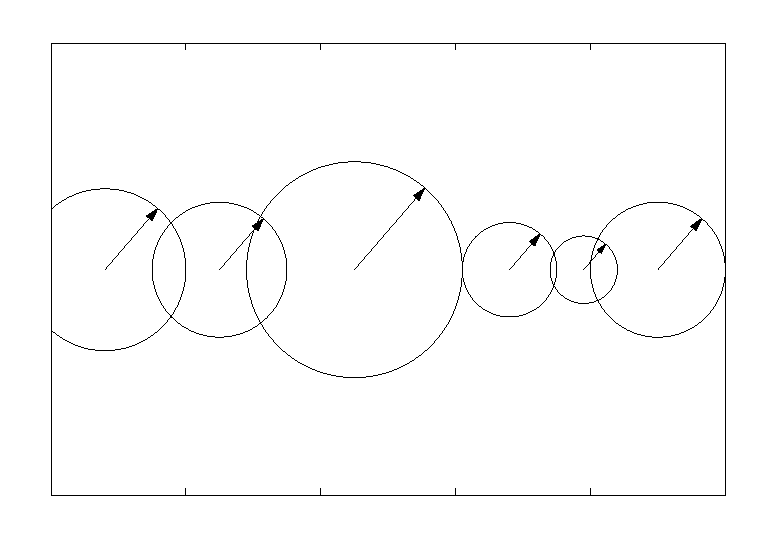
\includegraphics{Arrows}}%
    \gplfronttext
  \end{picture}%
\endgroup

\caption[Cousin's Theorem Depiction]{Cousin's Theorem states that there exists a finite subcover of a closed interval. For example, consider the interval $[1,2] \in \mathbb{R}$, then there exists a finite collection of circles (or more generally balls) of radii $\delta_i/2$ which spans the interval.}
\label{fig:arrows}
\end{figure}

Physically, we require the velocity potential to be continuous, and so the Hankel transform (and in fact all integral transforms) should preserve continuity, as shown in Theorem \ref{thm:continuity}.

\begin{theorem}
\label{thm:continuity}
$\mathcal{T}f$ is continuous if $\int_a^b |f(y)| dy < \infty$, and $K(x,y)$ is uniformly continuous on $[a,b]$.
\end{theorem}
\begin{proof}
For all $\varepsilon > 0$, choose $\delta : |x - x_0| < \delta$, so that $|K(x,y) - K(x_0,y)| < \varepsilon/M$, with $M = \int_a^b |f(y)| dy$. Then,
\begin{align*}
|(\mathcal{T}f)(x) - (\mathcal{T}f)(x_0)| &= \left| \int_a^b K(x,y)f(y) dy - \int_a^b K(x_0,y)f(y) dy \right| \\
&\leq \int_a^b |K(x,y) - K(x_0,y)||f(y)| dy \\
&< \int_a^b \frac{\varepsilon}{M} |f(y)| dy \\
&< \varepsilon,
\end{align*}
and $\mathcal{T}f$ is continuous.
\end{proof}

The conditions for Theorem \ref{thm:continuity} are automatically satisfied by Theorem \ref{thm:uniform} if $a$ and $b$ are finite, and $K$ is bounded and continuous.

\section{Hankel Transform}

The Hankel transform, named after the German mathematician Hermann Hankel, is quite common in cylindrically symmetric systems, such as ours, and arises from the eigenfunctions of Laplace's equation.

\begin{definition}[Hankel Transform]
\label{def:hanktrans}
The Hankel transform of a function $f(s)$ is given by
\begin{align*}
\Hank[\nu]{f}(\sigma) = \int_0^\infty f(s) J_\nu(s \sigma) s \, ds,
\end{align*}
where $J_\nu$ is the Bessel function of the first kind, of order $\nu \geq -\frac{1}{2}$, and $\sigma$ is a non-negative real variable.
\end{definition}

Notice too, that it directly follows from Definition \ref{def:hanktrans} that the Hankel transform is self-reciprocal.

\begin{corollary}[Inverse Hankel Transform]
\label{def:invhanktrans}
The Hankel transform is self-reciprocal, that is, the inverse Hankel transform is also given by Definition \ref{def:hanktrans}.
\end{corollary}
\begin{proof}
The Hankel transform is self-reciprocal
\begin{align*}
\iff f(s) &= \int_0^\infty \Hank[\nu]{f}(\sigma) J_\nu(s \sigma) \sigma \, d\sigma \\
\iff &= \int_0^\infty \int_0^\infty f(s') J_\nu(s \sigma) s' \, ds' J_\nu(s \sigma) \sigma \, d\sigma \\
&= \int_0^\infty f(s') s' \int_0^\infty J_\nu(s' \sigma) J_\nu(s \sigma) \sigma \, d\sigma \, ds' \\
&= f(s),
\end{align*}
by the orthogonality of the Bessel functions.
\end{proof}

However, only the order zero Hankel transform will be used in the analysis, so the $\nu$ shall be omitted and assumed zero, unless otherwise stated. Note that the kernel function of the Hankel transform is not $J_0 (s \sigma) s$, but in fact $\sqrt{s} J_0 (s \sigma)$, the other $\sqrt{s}$ factor gets absorbed into $f$. This is to ensure uniform continuity of the kernel (Lemma \ref{lem:Jcont}), and the continuity of the transform, while minimizing the constraint on $f$. As a consequence, we have the modified condition that $\int_0^\infty \sqrt{s}|f(s)| ds < \infty$.

\begin{lemma}
$\sqrt{s}J_0(s \sigma)$ is uniformly continuous on $[0,\infty)$.
\label{lem:Jcont}
\end{lemma}
\begin{proof}
Let $N$ be a sufficiently large number. By Theorem \ref{thm:uniform}, $\sqrt{s}J_0(s \sigma)$ is uniformly continuous on $[0,N]$. And on the interval $(N,\infty)$,
\begin{align*}
J_0(s \sigma) \rightarrow \sqrt{\frac{2}{\pi s \sigma}} \cos \left( s \sigma - \frac{\pi}{4} \right)
\end{align*}
asymptotically, and therefore $\sqrt{s}J_0(s \sigma)$ is uniformly continuous on $[0,\infty)$ since cosine is uniformly continuous everywhere by its periodicity.
\end{proof}

\begin{theorem}
The Hankel transform is continuous if $\int_0^\infty \sqrt{s}|f(s)| ds < \infty$.
\end{theorem}
\begin{proof}
Lemma \ref{lem:Jcont} shows the uniform continuity of the kernel, and $\int_0^\infty \sqrt{s}|f(s)| ds < \infty$ is a stronger condition than $\int_0^\infty |f(s)| ds < \infty$, thus by Theorem \ref{thm:continuity}, the Hankel transform is continuous.
\end{proof}

The following, and final theorem will be particularly useful for calculating the energy deposited to the neutron star.
\begin{theorem}
\label{thm:square}
The integral of the square of the Hankel transform weighted by $\sigma$ is equivalent to the integral of the square of the function weighted by $s$:
\begin{align*}
\int_0^\infty \Hank[\nu]{f}^2(\sigma) \sigma \, d\sigma = \int_0^\infty f^2(s)s \, ds.
\end{align*}
\end{theorem}

\begin{proof}
From the definition of the Hankel transform we have
\begin{align*}
\int_0^\infty \Hank[\nu]{f}^2(\sigma) \sigma \, d\sigma &= \int_0^\infty \int_0^\infty f(s) J_\nu(s \sigma) s \, ds \int_0^\infty f(s') J_\nu(s' \sigma) s' \, ds' \, \sigma \, d\sigma, \\
&= \int_0^\infty \int_0^\infty f(s) f(s') s \, s' \int_0^\infty J_\nu(s \sigma) J_\nu(s' \sigma) \sigma \, d\sigma \, ds \, ds', \\
&= \int_0^\infty f^2(s) s \, ds
\end{align*}
by the orthogonality of Bessel functions.
\end{proof}

\subsection{Applications of the Hankel Transform}

As previously noted, the Hankel transform arises from axisymmetric problems in cylindrical coordinates from the radial eigenfunction of Laplace's equation. Because of this, the Hankel transform along with the Laplace transform have many applications in solving partial differential equations in physics. Some examples include, but are not limited to, the free vibration of a circular membrane, the diffusion equation, acoustic radiation, or even the axisymmetric Cauchy-Poisson wave problem which shares many similarities with this work \cite{transforms}.

%\end{document}
